%!TEX root = ../thesis.tex


\begin{table}[]
\centering
\resizebox{\textwidth}{!}{%
\begin{tabular}{llll}
\hline
Method                & Description \\ \hline
execCommand           & Executes a command. \\
queryCommandEnabled   & Returns whether or not a given command can currently be executed. \\
queryCommandIndeterm  & Returns whether or not a given command is in the indeterminate state. \\
queryCommandState     & Returns the current state of a given command. \\
queryCommandSupported & Returns whether or not a given command is supported by the current document's range. \\
queryCommandValue     & Returns the value for the given command. \\ \hline
\end{tabular}
}
\caption{HTML Editing API}
\label{table:editing_mode_api}
\end{table}

\clearpage
\newpage

\begin{landscape}

  \begin{figure}[htb]
    \centerline{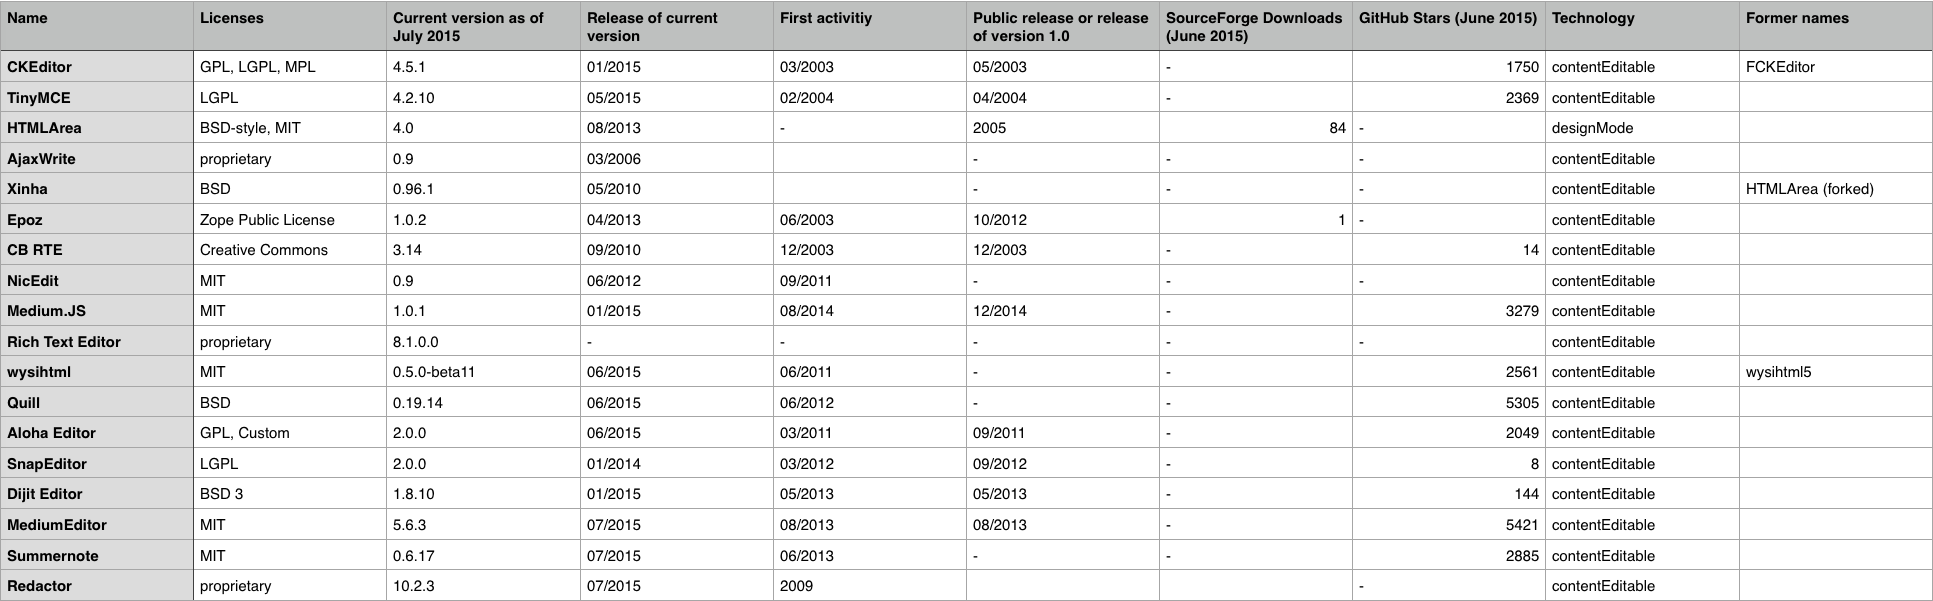
\includegraphics[width=\linewidth]{images/table-ce-editors.png}}
    \caption{Editors using HTML editing APIs}
    \label{fig:editors_editing_apis_table}
  \end{figure}
  
  \begin{figure}[htb]
    \centerline{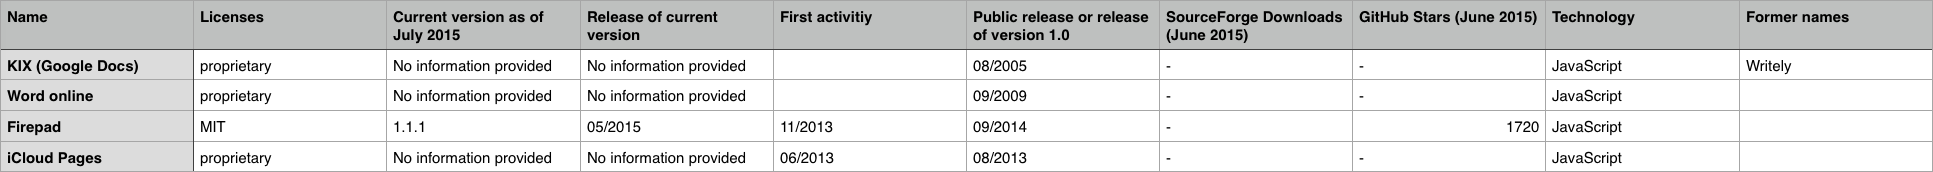
\includegraphics[width=\linewidth]{images/table-js-editors.png}}
    \caption{Editors not using HTML editing APIs}
    \label{fig:editors_not_editing_apis_table}
  \end{figure}
  
\end{landscape}


\clearpage
\newpage
